\chapter{Tutorial}
\label{ch:geolog-tutorial}

\noindent\draftmark\medskip

If you have operated an event-sourced system, you have already run
most of geolog's architecture on convention \cite{kleppmann21}. An
append-only log serves as the source of truth. Derived views are
rebuilt by replay. New capability arrives as new producers and
consumers, never as mutation of shared state. And everybody promises
not to write to the derived tables by hand. Kafka gives you the log,
Flink or Feldera maintains the views, a schema registry polices the
shapes, and the promises live in code review.

geolog takes that architecture and makes the promises structural. No
fold code that somebody wrote and everyone else must believe maintains
the derived views; the declared axioms \emph{entail} them instead, and
they can be recomputed and checked from the log alone. The chapter's
spine is one example, an order flow with two writers: views no single
writer can derive (\S\ref{sec:gt-views}--\ref{sec:gt-single}), merge
as set union plus re-derivation (\S\ref{sec:gt-merge}), the signed
commit log and what it can say that a broker cannot
(\S\ref{sec:gt-log}), schemas as data (\S\ref{sec:gt-schema}), and the
ground vocabulary (\S\ref{sec:gt-ground}). A worked example imported
from an independent project follows: the core theory of a proof
assistant, expressed whole, together with instructions for converting
its native data in both directions (\S\ref{sec:gt-alifib}). A
plain-dealing scorecard against the SQL stack you already run
(\S\ref{sec:gt-scorecard}) and the handoff to temporal claims
(\S\ref{sec:gt-onward}) close the chapter. Every transcript is
verbatim from a real run against the geolog-alpha repository (the
order flow against \path{examples/orders.geolog} and the
single-diagram crossing of \S\ref{sec:gt-alifib}, last re-executed
2026-07-30 against the import-era tree; the corpus-scale
measurements behind \S\ref{sec:gt-alifib} executed 2026-07-27); the
receipts sit at this chapter's source tail.

\section{Views you do not maintain}
\label{sec:gt-views}

Here is the domain, whole. Two writers will keep logs against it: a
storefront (payments, cancellations) and a warehouse (allocations,
shipping records).

\begin{Verbatim}[fontsize=\small,frame=leftline,rulecolor=\color{accentmid},framesep=3mm,xleftmargin=3mm]
theory Orders {

  Order    : Set;
  Shipment : Set;

  // Events -- asserted rows, the writers' ground truth.
  Placed    : [o: Order] -> Prop;
  Paid      : [o: Order] -> Prop;
  Allocated : [o: Order] -> Prop;
  Cancelled : [o: Order] -> Prop;

  // Views -- derived rows, never asserted by a writer...
  Shippable : [o: Order] -> Prop;

  // ...except ShippedVia, which writers MAY also assert (a recorded
  // manifest); where no record exists, the chase invents the witness.
  ShippedVia : [o: Order, s: Shipment] -> Prop;

  chase ax/ship/ready : forall o : Order.
    [o: o] Paid, [o: o] Allocated |- [o: o] Shippable;

  chase ax/ship/manifest : forall o : Order.
    [o: o] Shippable |- exists s : Shipment. [o: o, s: s] ShippedVia;

  chase ax/manifest/unique : forall o : Order, s1 : Shipment, s2 : Shipment.
    [o: o, s: s1] ShippedVia, [o: o, s: s2] ShippedVia |- s1 = s2;

  report ax/no/zombie : forall o : Order, s : Shipment.
    [o: o] Cancelled, [o: o, s: s] ShippedVia |- false;
}
\end{Verbatim}

Read \texttt{ax/ship/ready} the way you would read a view definition,
because that is what it is:

\begin{Verbatim}[fontsize=\small,frame=leftline,rulecolor=\color{accentmid},framesep=3mm,xleftmargin=3mm]
CREATE MATERIALIZED VIEW shippable AS
  SELECT o FROM paid INTERSECT SELECT o FROM allocated;
\end{Verbatim}

\noindent The \texttt{chase} mark plays the role of \texttt{CREATE}
here. It opts the sequent into \emph{firing}, which is to say into
deriving rows. A \texttt{report} mark, or no mark at all (unmarked
means \texttt{report}), would instead make the same sequent a checked
constraint, judged and never fired. The join stays identical; what
changes is who owes whom what. A materialized view comes out of the
query you wrote together with the engine's maintenance code, and it
contains whatever that code computed. A geolog view, by contrast, is a
logical consequence. The chase computes the \emph{least fixpoint} of
the axioms over the asserted rows: every row the axioms force, and no
row they do not. Anything that can replay the log and read the theory
can then re-derive and audit every row, with its provenance. In the
SQL world the nearest neighbours are Feldera and the DBSP line of work
\cite{budiu22}, and the kinship is genuine: declarative view
definitions, incremental maintenance with a correctness story, replay
from a log. What differs is the view language itself. A SQL view
computes what its query says; a geolog view is an entailment in
geometric logic \cite[Part~D1]{johnstone2002}, the fragment of
first-order logic whose sequents have a conjunction of atoms as
premise and a disjunction of existentially quantified conjunctions as
conclusion. That fragment is why the other three axioms above (an
existential, an equality, and a denial) are ordinary view
definitions here, while over there they are not expressible as views
at all. Those three carry the rest of this chapter.

Two caveats, up front. The first is maintenance. Feldera's engine is
incremental to its bones, and at production scale that maturity is
real (\S\ref{sec:gt-scorecard}). In this preview, geolog's chase
evaluation is a deliberately naive reference implementation,
differentially tested against an independent engine and built to be
right rather than fast; incremental maintenance ships today only for
its violation views, where the failing set is kept current under row
deltas and never recomputed from scratch. The second is expressiveness,
and it cuts the other way. Aggregates such as \texttt{SUM} and
windowed rates, the bread of streaming SQL, are not native vocabulary
in the geometric fragment. Counting enters through explicit
constructions or through the ground seam (\S\ref{sec:gt-ground}), and
where your computation is aggregate-shaped, today the SQL stack simply
wins.

\section{One writer at a time}
\label{sec:gt-single}

The two writers' logs live as two \texttt{instance} blocks in the
same file; in the durable pipeline each would instead be a stream of
signed commits (\S\ref{sec:gt-log}). The storefront saw payments and a
cancellation, and it holds the carrier's tracking record for order
\texttt{o1}. The warehouse allocated stock for both orders, the
cancellation not having reached it, and it holds its own record of the
same shipment, the printed label:

\begin{Verbatim}[fontsize=\small,frame=leftline,rulecolor=\color{accentmid},framesep=3mm,xleftmargin=3mm]
instance Storefront : Orders {
  o1, o2 : Order;
  sf_record : Shipment;

  [o: o1] Placed;  [o: o1] Paid;
  [o: o2] Placed;  [o: o2] Paid;
  [o: o2] Cancelled;

  [o: o1, s: sf_record] ShippedVia;
}

instance Warehouse : Orders {
  o1, o2 : Order;
  wh_label : Shipment;

  [o: o1] Allocated;
  [o: o2] Allocated;

  [o: o1, s: wh_label] ShippedVia;
}
\end{Verbatim}

Chase each log alone (\texttt{--instance} selects blocks):

\begin{Verbatim}[fontsize=\small,frame=leftline,rulecolor=\color{accentmid},framesep=3mm,xleftmargin=3mm]
$ geolog chase examples/orders.geolog --instance Storefront
  ⋮
  Shippable — 0 rows (0 seeded, 0 derived)
  ShippedVia — 1 row (1 seeded, 0 derived)
    [o: o1, s: sf_record] ShippedVia
fixpoint: reached, no judgements — the model is saturated.
$ echo $?
0
\end{Verbatim}

\noindent The warehouse's run is symmetric: no \texttt{Paid}
rows, so again no \texttt{Shippable}, and exit 0. Notice what clean
means here. \emph{Each writer's log is locally consistent.} The
storefront knows \texttt{o2} is cancelled but sees no shipment for it,
and the warehouse sees no cancellation at all. Every partial view is
innocent. If the two logs were Kafka partitions consumed by separate
services, each service would be reporting green.

\section{Merge is set union plus re-derivation}
\label{sec:gt-merge}

Now merge. Merging replicas in geolog takes no protocol. The commit
bag is a set, union is union, and the chase re-derives. Run without
\texttt{--instance} and the file's blocks seed as their union. Element
names shared across blocks denote the same element, the CLI's
small-scale stand-in for the content-addressed identity of
\S\ref{sec:gt-log}:

\begin{Verbatim}[fontsize=\small,frame=leftline,rulecolor=\color{accentmid},framesep=3mm,xleftmargin=3mm]
$ geolog chase examples/orders.geolog
sorts:
  Order — 2 elements (2 seeded)
  Shipment — 2 elements (2 seeded, 1 invented by the chase,
                         1 merged by congruence)
  merged: sf_record = wh_label
relations:
  ⋮
  Shippable — 2 rows (0 seeded, 2 derived)
  + [o: o1] Shippable
  + [o: o2] Shippable
  ShippedVia — 2 rows (1 seeded, 1 derived)
    [o: o1, s: sf_record=wh_label] ShippedVia
  + [o: o2, s: ?Shipment.0] ShippedVia
judgements (1):
  denial violated: ax/no/zombie at [o: o2, s: ?Shipment.0]
$ echo $?
1
\end{Verbatim}

Four things happened, and they are four fifths of this database's
distinctive behaviour, so take them one at a time.

\paragraph{The union derived what neither log could.}
\texttt{Shippable} was empty in both single-writer runs, and the
merged run derives it for both orders, because
\texttt{ax/ship/ready}'s premise spans the two logs. That much is the
ordinary magic of any log-merging system; a Feldera pipeline consuming
both topics would derive the same join. What it did not require was a
pipeline topology. The axiom was already the join, and \emph{any}
subset of commits chases to its own well-defined fixpoint.

\paragraph{The two writers' records became one shipment.}
The storefront's \texttt{sf\_record} and the warehouse's
\texttt{wh\_label} are two elements naming, as it turns out, one real
shipment. \texttt{ax/manifest/unique} says as much: a shipment is one
shipment. The engine's congruence closure \emph{identifies} the two
elements, and the report prints the merged element as
\texttt{sf\_record=wh\_label}. Contrast the CRDT discipline you may
run on Kafka-adjacent state stores. There, convergence is bought by
designing every value as a lattice and every merge as a join, per
type, by hand, in advance. Here identity is a \emph{logical} matter,
decided by the theory's equality axioms and computed by congruence,
and it composes with everything else the axioms say. It is also a mode
\emph{choice}, made where the axiom is written.
\texttt{ax/manifest/unique} is \texttt{chase}-marked
deliberately, because identification is this axiom's job;
\texttt{report}-marked, the same sequent would instead judge two
distinct records as a violation, which is the right reading in a
domain where identity is content and merging would invent facts. (When
two elements merge, everything known about either transfers to the one
survivor. Judging \texttt{ax/no/zombie} against the invented witness
below already relies on that.)

\paragraph{The chase invented a witness.}
Order \texttt{o2} became \texttt{Shippable}, and
\texttt{ax/ship/manifest} demands that a shipment exist for every
shippable order. No writer recorded one, so the chase minted
\texttt{?Shipment.0}, a fresh element about which nothing is known
except what the axiom forces. This is the \emph{restricted chase}:
existentials invent a witness only where no witness already exists
(order \texttt{o1}, which had records, got no invention). If you know
database theory you recognize tuple-generating dependencies and the
chase from the classical literature
\cite{fagin2005data,deutschnashremmel2008}; if you know event-sourced
systems, read it as the database itself filing the missing follow-up
event, typed, provenance-tracked, and only when entailed.

\paragraph{The violation surfaced only at the merge, and was
reported rather than resolved.}
Both logs were locally clean. Their union contains a cancelled order
with a shipment, and \texttt{ax/no/zombie} forbids precisely that. The
chase does not reject the merge, since there is nothing to reject; the
union of two sets of commits is a set of commits. Nor does it pick a
loser or roll anything back. It reports the judgment, with the
axiom's name and the witnessing binding, and exits nonzero. That
posture is the event-sourcing one, held formally: \emph{invalid states
are representable, detected, and repaired by further ordinary
commits} --- a compensating cancellation of the shipment, a voiding
of the cancellation, whichever the workflow's owner chooses. What the
database contributes is that ``invalid'' is a theorem rather than a
code path someone remembered to write, and that the judgment itself
is data an agent can act on. (Where an axiom's conclusion offers a
genuine \emph{choice} of repairs, a disjunctive head, the engine
likewise picks nothing, and the judgment carries the menu. The engine
calls these branch points; this example's judgments are denials,
menus of length zero.)

If you have fought a Kafka consumer-group rebalance that replayed a
partition into a half-updated store, or reconciled two services'
databases after a network partition, this section is the pitch. Merge
here is set union, and so it is \emph{always} defined, order-free, and
idempotent; and every consequence of the merged log, including its
violations, can be re-derived by anyone from the log alone.

\section{The log is the ground truth}
\label{sec:gt-log}

Everything so far ran from a source file, because this is a tutorial.
In geolog, ``the facts'' take durable form as a log of \emph{commits}:
content-addressed, ed25519-signed envelopes whose payloads carry just
the kind of rows you have been reading, and whose causal dependencies
are part of the signed content. Crossing from the file to that log is
one verb:

\begin{Verbatim}[fontsize=\small,frame=leftline,rulecolor=\color{accentmid},framesep=3mm,xleftmargin=3mm]
$ geolog seal examples/orders.geolog --store orders-store --repro
repro-signed (public seed "geolog-seal-repro-v1" — reproducibility, not authority)
sealed examples/orders.geolog: 1 theory, 4 axioms, 197 revision ops
revision commit:  b128db74d04f92bb0fdc5aec5a26f1d67b5504ba9289a7e888b487c1ee232aa4
C1 revision hash: c7de71b56edc728bc65daba559d3e3f1b0bf32bf2030689de4e1b69d64066f7f
seal commit:      e69f4611e367e91c8509731fc04f349ccf0b18beef0ea1f87788ce6351505a59
store: genesis minted, comparisons minted, revision minted, seal minted
\end{Verbatim}

\noindent The theory's declarations compile to meta-schema rows
(\S\ref{sec:gt-schema}), the rows seal into a signed revision commit,
and the store on disk now holds the envelope shapes the storage
crates document and test (\path{geolog-envelope}, \path{geolog-store},
and \path{geolog-sync}, each with its differential partner named in
its README). Sealing is deterministic: re-running the command reports
every commit \texttt{already present}, and \texttt{--repro} signs
with a public seed so that the hashes above reproduce from a fresh
clone (reproducibility, as the tool says, not authority).
\texttt{geolog check --store} and \texttt{geolog chase --store} then
run the strata you already know over the sealed source instead of the
file, after signature verification and a coherence gate; the
reference manual's CLI section (\S\ref{sec:gr-cli}) walks the whole
verb family, \texttt{extract} and \texttt{load} included.

The architecture invites a comparison. A Kafka topic with infinite
retention is also an append-only ground truth, and replay-rebuilt
views are also disposable. Three differences are worth having words
for.

\paragraph{The log forms a set rather than a sequence.} A topic is an
ordered sequence per partition, and that order carries real weight:
consumers coordinate offsets, rebalances are delicate, cross-partition
order is undefined. A geolog commit bag is unordered. Causality is
explicit, since each commit names its dependencies by hash, and
derived state does not depend on admission order. The repository's
battery includes a rebuild invariant that diffs
incrementally-maintained state against a from-scratch replay, and a
divergence is a release-blocking bug. ``Replays in any order to the
same fixpoint'' is the property that made \S\ref{sec:gt-merge}'s merge
a non-event.

\paragraph{Writers are cryptographic identities, and equivocation is
detectable.} A broker will happily append whatever a producer sends,
and if a compromised or buggy writer tells two consumers two different
stories, nothing in the topic model even states the offence. geolog
commits are signed and content-addressed, and a writer's log is a
hash-linked chain. A writer that forks its own history, which is to
say equivocates, is detected \emph{structurally} at sync time, from
the bytes alone, with no consensus protocol and no quorum; the same
mechanism makes CRDTs Byzantine fault tolerant in Kleppmann's
construction \cite{kleppmann22}. (The repository's envelope crate
ships the demonstration as a test: two signed commits claiming the
same chain position are the offence, exhibited and caught.)

\paragraph{Validity is per-commit and logical.} Because consequences
and violations re-derive from any subset of the log, ``which commits
does this judgment implicate'' is a well-posed question. The
provenance machinery exists in the engine, so that every derived row
and every invented element carries its firing history; and the
engine's validity layer (\path{geolog-chase/validity} in the
repository) makes the per-commit verdict itself durable: it replays a
commit's inclusive causal closure into a content-addressed snapshot
and folds one verdict per commit --- clean, judged with its
violations attached, or a named abstention (\texttt{pending},
\texttt{unsupported}, \texttt{indeterminate}), never a silent skip
--- with rebuild-order and cross-process determinism tested down to
byte-identical snapshot bytes, so two replicas that judge the same
commit publish the same judgment. Its first version replays a
deliberately narrow fragment (one theory revision per closure,
unmarked axioms only), and the tutorial CLI does not surface the
pipeline yet.
Capability-scoped authorization over the same substrate, meaning who
may extend which theory and assert into which relation, is likewise
arriving as an algebra over commits rather than as an ACL bolted on
beside them (\path{geolog-caps} ships the algebra today; enforcement
at the store boundary is design tense).

And the repository eats its own cooking: its committed theory
goldens are themselves stored as signed artefacts, minted by a
public, documented ceremony, and

\begin{Verbatim}[fontsize=\small,frame=leftline,rulecolor=\color{accentmid},framesep=3mm,xleftmargin=3mm]
cargo run -q -p geolog-ceremony -- verify --root theories
\end{Verbatim}

\noindent re-derives them byte-identically from their committed
listings and verifies the committed signatures, the golden-drift alarm
that runs in every CI pass.

\section{Schema is data}
\label{sec:gt-schema}

The Quick Start ended with \texttt{geolog rows}. The theory you write
is itself rows: \texttt{Theory}, \texttt{Sort}, \texttt{Fun}, and
\texttt{Field} elements in the \emph{meta-schema}, the schema language
that is a geolog theory like any other. In an event-sourced shop this
should land as the resolution of a familiar irritation, the schema
registry. Avro or protobuf schemas live \emph{beside} the topics, in a
registry with its own evolution rules (backward, forward, or full
compatibility), its own versioning, and its own failure modes: a
second database whose consistency with the first is everyone's job and
no one's.

In geolog there is no second database. A theory arrives as a
\emph{revision}, a sealed batch of meta-schema rows, committed,
signed, and content-addressed just like every other commit, with its
dependencies named. Extending a schema means a further revision that
depends on the first. Two independent extensions merge like any other
commits, by set union, with the chase over the meta-schema re-deriving
the combined signature. And ``what did the schema look like when this
row landed'' is a query over the same log as the row. Annotations
follow the same pattern instead of a special mechanism: the
repository's worked units-of-measure theory decorates an existing
theory's declarations with dimension gradings from the \emph{outside},
as ordinary relation rows over \texttt{Fun} and \texttt{Sort}
elements, without touching the annotated theory's bytes.

Here is what ships today in the alpha repository: the meta-schema
itself, the genesis golden of \S\ref{sec:gt-log}'s ceremony; the
reference row listings and their generators for the worked theories
under \path{theories/}; the theory-to-rows compiler and the
sealed-revision conformance loader, with byte-identical round-trips on
the committed corpora and loud rejections collected per rule; and the
revision-level machinery, namely declaration indexes, signature
hashes, and a programmatic revision-body builder. The \texttt{geolog
rows} verb you ran is a faithful \emph{view} of the declaration slice,
and \texttt{geolog seal} runs the same compilation for keeps: the
transcript of \S\ref{sec:gt-log} sealed the order theory as a signed
revision of 197 meta-schema operations. Cross-revision
\texttt{extends}, parameterized theories, and instances as
first-class elements are specified in the ruled design documents and
arrive as that store grows; the tutorial's single-file
\texttt{extends}, which the CLI does accept, is the in-file shadow of
that mechanism.

\section{Ground vocabulary: decided, not stored}
\label{sec:gt-ground}

Everything so far has been finite rows over declared sorts. Real
domains want numbers, timestamps, and comparisons, vocabulary whose
extension no log could store (\emph{every} pair of rationals with $a
\le b$?) and no chase should enumerate. geolog's answer is the
\emph{ground seam}. Relations and functions over immutable carriers
are declared as theory rows like everything else, but \emph{decided}
by registered procedures: exact arbitrary-precision rational
arithmetic, and calendar arithmetic whose semantics are documented and
tested against PostgreSQL's (\texttt{date} + \texttt{interval}
behaviour, chosen precisely so a SQL practitioner's instincts transfer
and the corner cases are somebody's published corner cases rather than
ours).

Two disciplines make the seam trustworthy rather than a trapdoor. The
first is \emph{refusal over guessing}. Ground vocabulary an
application declares but no provider implements does not default,
approximate, or silently empty; a plan that cites it cannot even be
expressed, and the refusal names the atom. (A division's graph simply
contains no row for a zero divisor, so ``divide by zero'' is
underivability rather than an exception.) The second is \emph{the lane
law}: an accelerated implementation may change \emph{cost}, never
\emph{verdicts}. Every fast lane is conformance-gated against the
always-on exact reference, and a lane that cannot pass its battery
does not dispatch. If your mental model of database extension points
is user-defined functions, hold on to this contrast: a UDF is trusted
code in the query path, whereas a ground provider is an untrusted
proposal bound to a declared signature, adjudicated by the engine,
with an exact reference underneath it.

(The tutorial's CLI bridge does not yet reach the ground seam.
\texttt{geolog chase} today covers declared sorts and
\texttt{Prop}-valued relations, and it says so loudly when a theory
wants more. The engine-level seam, the exact-rational floor, and the
calendar corpus are in the repository under test; the worked
Petri-net theory shows the discipline of doing real arithmetic
\emph{without} the seam, as chase-derived rows over an explicit number
ladder.)

\section{Worked example: alifib in geolog}
\label{sec:gt-alifib}

Everything in this chapter so far was designed to teach this chapter.
This section imports a structure that was not. \emph{alifib}
\cite{alifib} is an experimental programming language and interactive
proof assistant founded on higher-dimensional rewriting, developed by
Amar Hadzihasanovic together with Alex Kavvos within ARIA's
Safeguarded AI programme; its mathematics is Hadzihasanovic's theory
of directed complexes and molecules \cite{hadzihasanovic24a}, and its
data structures grew out of joint work with Diana Kessler
\cite{hadzihasanovic23}. In alifib a type is a directed cell complex;
a value is a \emph{diagram} drawn in that complex; and a computation
on $n$-dimensional data is itself a diagram, one dimension up.
Running a program builds a witness of the whole computation, a
higher-dimensional term you can inspect, paste into larger diagrams,
and reason about; the project calls the property \emph{computational
transparency}. Rewrite rules are ordinary generators one dimension up,
so there is no separate sort of rules anywhere in the language, and an
execution trace is a term like any other.

Two of this chapter's themes meet in it, and it forces a third; that
is why it earns a section. First, schema as data
(\S\ref{sec:gt-schema}) at full
stretch: the whole proof theory lands as one ordinary geolog theory,
seven sorts, thirty-eight functions and relations, twenty-four axioms,
with no extension to the meta-schema at all. Second, decided rather
than stored (\S\ref{sec:gt-ground}): every judgment the alifib engine
computes over its finite combinatorial data --- whether a paste is
legal, whether a boundary pair is round, whether an incidence table
matches a realized shape --- enters the theory as a side-condition
relation whose evaluator is the engine itself, the ground-seam
discipline pointed at a full external prover rather than at rational
arithmetic. Third, the forced one: the geometric fragment offers no
negation in premises, and a theory of cell complexes keeps wanting one sentence of that shape (``this cell has no
coface''). The stored-complement idiom below carries that sentence
without leaving the fragment.

The theory ships as \path{theories/Alifib.geolog} in the geolog-alpha
repository, and its opening \texttt{import} header is the
decided-versus-stored split of \S\ref{sec:gt-ground} written down:
the file imports its eight engine-decided judgments from the
\texttt{alifib} namespace (each import classifying that relation
\texttt{side-condition} --- decided by a bounded external procedure),
and every relation it declares without importing is
\texttt{ordinary}, the default. The check verb runs green on it:

\begin{Verbatim}[fontsize=\small,frame=leftline,rulecolor=\color{accentmid},framesep=3mm,xleftmargin=3mm]
$ geolog check theories/Alifib.geolog
[1/5] parse + normalize + lint: theories/Alifib.geolog @ 2e60dd6 (452 lines)
      1 theories; 24 axioms (0 moves; aux helpers: none)
[2/5] geometric linter: CLEAN
  ⋮
[5/5] instance conformance: no instance blocks in this file
modes: 6 chase · 18 report (18 by the unmarked default) · 0 refuse
  ⋮
CHECK: GREEN
$ echo $?
0
\end{Verbatim}

\noindent The excerpts below are the teaching spine, roughly a third
of the theory; the axioms not shown (execution traces as first-class
terms; roundness of each generator's boundary pair, the shape
condition on a single cell; the remaining three sequents of the
boundary-parity family; uniqueness of a cell's coordinate; homing of
boundary rows and map images) repeat the three patterns you are about
to see. The theory splits into two tiers, the syntax of assemblies
and the incidence data of the shapes they realize, and the walk takes
them in order. One caveat before it starts: the tutorial CLI's
\texttt{rows} and \texttt{chase} verbs do not reach this theory yet
--- its element-valued function symbols are engine IR the current
chase bridge does not carry --- and both refuse loudly, each naming
its workaround in the refusal. The transcripts here therefore ride
\texttt{check}, \texttt{census}, and the conversion tools, and the
excerpts themselves are kept faithful by construction: concatenated in
source order they form a well-formed theory that \texttt{geolog check}
accepts (the receipt at this chapter's source tail records that run).

\subsection{Paste trees as constructor rows}
\label{sec:gt-alifib-tier1}

\begin{Verbatim}[fontsize=\small,frame=leftline,rulecolor=\color{accentmid},framesep=3mm,xleftmargin=3mm]
theory Alifib {

  AType : Set;   // a type: a directed complex, elaborated
  Gen   : Set;   // one generator (cell) of a type; a rewrite
                 // rule is a Gen one dimension up
  Diag  : Set;   // a diagram AS ASSEMBLY -- a binary paste tree
  AMap  : Set;   // a map between types (generator-to-diagram images)
  Cplx  : Set;   // a materialized oriented graded poset
  Cell  : Set;   // one cell of a Cplx
  // (the seventh sort, Trace, records executions: a witness diagram
  //  one dimension up, with its endpoints)

  Gen/type : Gen -> AType;
  Gen/dim  : Gen -> Nat;
  Gen/src  : Gen -> Diag;   // PARTIAL: absent iff dim = 0 --
  Gen/tgt  : Gen -> Diag;   // a 0-cell has no boundaries

  dGen   : [g: Gen] -> Diag;                    // a single cell
  dPaste : [k: Nat, l: Diag, r: Diag] -> Diag;  // l #k r
\end{Verbatim}

alifib builds diagrams by \emph{pasting}: \texttt{l \#k r} glues two
diagrams along their shared $k$-dimensional boundary, and the engine
stores a diagram as its assembly history, a binary tree of pastes over
single-cell leaves. The two constructors above mirror that
representation without loss. Because \texttt{dPaste} is a function ---
one value per argument tuple, an equality the chase maintains by
merging --- two occurrences of the same tree denote one \texttt{Diag}
element, and structurally equal assemblies are shared: the engine's
own pointer-sharing, recovered as identity semantics. What a
\texttt{Diag} element is \emph{not} is a diagram up to isomorphism:
two trees can realize isomorphic diagrams and remain distinct
elements, related by a declared side-condition (\texttt{alifib\_iso},
in the full theory). That choice matches the engine, which stores
assemblies and \emph{computes} isomorphism, and it is the honest one
for a database: identity of stored data stays structural, and the
quotient stays a judgment.

Partiality needs no apparatus. A 0-cell has no boundaries, so
\texttt{Gen/src} simply has no row for it; there is no nullable column
and no sentinel: a boundary a generator lacks is a row nobody asserts,
and the axioms only ever demand what presence owes. The same
convention carries map holes below.

Everything the engine \emph{decides} about these trees enters as
side-condition relations, and the theory \emph{demands} the judgments
where they are owed:

\begin{Verbatim}[fontsize=\small,frame=leftline,rulecolor=\color{accentmid},framesep=3mm,xleftmargin=3mm]
  alifib_wf       : [d: Diag] -> Prop;   // realizes to a molecule
  alifib_pastable : [k: Nat, l: Diag, r: Diag] -> Prop;

  ax/wf/diag : forall d : Diag.
    |- [d: d] alifib_wf;

  ax/wf/paste : forall k : Nat, l : Diag, r : Diag, d : Diag.
    d = [k: k, l: l, r: r] dPaste
    |- [k: k, l: l, r: r] alifib_pastable;
\end{Verbatim}

\noindent Read \texttt{ax/wf/paste} as a well-formedness debt: every
asserted paste owes a pastability judgment, and the judgment is
discharged by evaluation, not by chase derivation --- each of these
relations is imported at the top of the file, which classifies it
\texttt{side-condition}, and the bounded external procedure behind
them is the alifib engine. The
refusal discipline of \S\ref{sec:gt-ground} carries over unchanged:
absent the engine, a plan citing these atoms cannot be expressed,
and nothing defaults to true.

One derived view shows the chase doing for proof theory what it did
for order flow. Which generators --- hence which rewrite rules ---
does a diagram use?

\begin{Verbatim}[fontsize=\small,frame=leftline,rulecolor=\color{accentmid},framesep=3mm,xleftmargin=3mm]
  Diag/uses : [d: Diag, g: Gen] -> Prop;

  chase ax/uses/gen : forall g : Gen, d : Diag.
    d = [g: g] dGen
    |- [d: d, g: g] Diag/uses;

  chase ax/uses/paste_l : forall k : Nat, l : Diag, r : Diag, d : Diag, g : Gen.
    d = [k: k, l: l, r: r] dPaste, [d: l, g: g] Diag/uses
    |- [d: d, g: g] Diag/uses;
\end{Verbatim}

\noindent (Its mirror \texttt{ax/uses/paste\_r} walks the right
subtree.) This is the \texttt{Shippable} of the proof theory: a table
nobody writes, entailed by structure, answering the question a proof
library wants indexed --- which rules does this proof depend on?

\subsection{Incidence, and maximality without negation}
\label{sec:gt-alifib-tier2}

A paste tree is a recipe. The shape it realizes is an \emph{oriented
graded poset}: cells graded by dimension, each cell covering its faces
with one of two signs, input or output. Chapter~\ref{ch:qtsl-scomplexes}
develops the S-complex vocabulary this book uses for such data and
notes that oriented graded posets embed as its Boolean instance; here
that instance appears as concrete rows. A materialized shape is a
\texttt{Cplx}; its cells carry a grade and an index within the grade
(the engine's canonical, normalization-derived order), and the two
signed covering relations land as two ordinary relations:

\begin{Verbatim}[fontsize=\small,frame=leftline,rulecolor=\color{accentmid},framesep=3mm,xleftmargin=3mm]
  Cell/cplx : Cell -> Cplx;
  Cell/dim  : Cell -> Nat;   // grade
  Cell/idx  : Cell -> Nat;   // index within the grade

  BdryIn  : [hi: Cell, lo: Cell] -> Prop;   // lo is an input face of hi
  BdryOut : [hi: Cell, lo: Cell] -> Prop;   // ... an output face

  ax/scx/sign_disjoint : forall hi : Cell, lo : Cell.
    [hi: hi, lo: lo] BdryIn, [hi: hi, lo: lo] BdryOut
    |- false;

  ax/scx/d2_pp : forall z : Cell, y : Cell, x : Cell.
    [hi: z, lo: y] BdryOut, [hi: y, lo: x] BdryOut
    |- exists w : Cell. [hi: z, lo: w] BdryOut, [hi: w, lo: x] BdryIn
    or exists v : Cell. [hi: z, lo: v] BdryIn, [hi: v, lo: x] BdryOut;
\end{Verbatim}

\noindent \texttt{ax/scx/sign\_disjoint} is a denial in the style of
\texttt{ax/no/zombie}: one sign per covering edge. The second axiom is
new territory. It is one quarter of the boundary-parity law, the
sign-aware face of $\partial \circ \partial = 0$: every two-step
signed path admits a two-step path of the opposite parity class
between the same endpoints. Its conclusion holds a genuine
disjunction, so the axiom is not chase-eligible --- there is no least
fixpoint to compute when the theory offers a choice --- and the engine
treats it exactly as \S\ref{sec:gt-merge} treated repairs: as a
judgment carrying a menu. Back there the menus had length zero; this
one has length two, and it earns its keep as a checked structural law
rather than a derivation rule (the reference manual's account of
per-axiom modes is \S\ref{sec:gr-chase-modes}). The law is not
hypothetical housekeeping: exporting all twenty-two example files
alifib ships, with included modules and every generator and named
diagram materialized, yields 37{,}988 complexes, and sign-disjointness
and the parity law hold across them with zero exceptions (receipt at
the chapter tail).

Now the idiom this section promised. ``$x$ is maximal'' means ``$x$
has no coface'', and that sentence wants negation in a premise, which
the geometric fragment deliberately lacks. Store the complement
instead:

\begin{Verbatim}[fontsize=\small,frame=leftline,rulecolor=\color{accentmid},framesep=3mm,xleftmargin=3mm]
  Cell/top     : Cell -> Prop;   // asserted: maximal (no coface)
  Cell/covered : Cell -> Prop;   // derived: has a coface

  chase ax/cell/covered_in : forall hi : Cell, lo : Cell.
    [hi: hi, lo: lo] BdryIn
    |- lo Cell/covered;

  chase ax/cell/covered_out : forall hi : Cell, lo : Cell.
    [hi: hi, lo: lo] BdryOut
    |- lo Cell/covered;

  ax/cell/top_not_covered : forall c : Cell.
    c Cell/top, c Cell/covered
    |- false;

  ax/cell/top_or_covered : forall c : Cell.
    |- c Cell/top or c Cell/covered;
\end{Verbatim}

\noindent Three moves. \emph{Generation}: \texttt{Cell/covered} is an
ordinary monotone view, derived from the boundary rows.
\emph{Exclusivity}: a denial keeps the asserted mark and the derived
view disjoint. \emph{Coverage}: a disjunctive law says every cell
falls on one side or the other --- judged, like the parity law, never
fired. Between them, ``maximal'' becomes queryable vocabulary, its
complement kept disjoint by the denial and exhaustive by the
disjunction, and no premise ever had to say \emph{not}. The pattern is
general; alifib merely needs it constantly, because boundaries of
pasting diagrams are defined through maximality.

\subsection{Maps, holes, and the axiom that must not fire}
\label{sec:gt-alifib-maps}

An alifib map assigns, to each generator of a domain type, a diagram
in a codomain type; alifib's proof workflow builds such maps
interactively, leaving \emph{holes} --- unassigned generators --- to be
filled as the proof progresses. In rows, a hole costs nothing:

\begin{Verbatim}[fontsize=\small,frame=leftline,rulecolor=\color{accentmid},framesep=3mm,xleftmargin=3mm]
  AMap/src : AMap -> AType;
  AMap/img : [g: Gen, m: AMap] -> Diag;   // PARTIAL: a hole is an
                                          // absent row
  AMap/total : AMap -> Prop;              // asserted mark

  ax/map/total : forall m : AMap, s : AType, g : Gen.
    m AMap/total, s = m AMap/src, s = g Gen/type
    |- exists i : Diag. i = [g: g, m: m] AMap/img;
}
\end{Verbatim}

\noindent Filling a hole is an ordinary append --- one new
\texttt{AMap/img} row --- so an interactive proof session is
event-sourced by construction, and ``what did this map look like
before the fill'' is a replay question like any other. The axiom is
the interesting resident. \texttt{ax/map/total} is chase-eligible on
its face: single disjunct, an existential the restricted chase knows
how to witness. Firing it would be a disaster in slow motion. The
chase would mint a fresh, contentless \texttt{Diag} for every open
hole of every map marked total, ``satisfying'' totality by inventing
images that mean nothing --- when what totality means for user data is
a \emph{judgment} that the user's own fills eventually discharge.
So the axiom stays report-marked, a checked debt rather than a
generator (one of the eighteen \texttt{report}s in the check
transcript above), and the invented-witness power of
\S\ref{sec:gt-merge} stays
where it belongs: on axioms whose existentials denote obligations the
database itself owns, like \texttt{ax/ship/manifest}'s missing
shipment. Choosing per axiom, in the source, with the default on the
safe side, is what the mode marks are \emph{for}.

\subsection{One diagram, end to end}
\label{sec:gt-alifib-e2e}

Here is a complete alifib type, small enough to watch cross the seam
whole. Two composable arrows, a third arrow, and one 2-cell rewriting
the pasted path into it (juxtaposition is alifib's shorthand for
pasting along the shared boundary of highest shared dimension; here
\texttt{f g} abbreviates \texttt{f \#0 g}):

\begin{Verbatim}[fontsize=\small,frame=leftline,rulecolor=\color{accentmid},framesep=3mm,xleftmargin=3mm,samepage=true]
@Type
Compose <<= {
    x, y, z,
    f: x -> y,
    g: y -> z,
    h: x -> z,
    step: f g -> h
}
\end{Verbatim}

\begin{figure}[htbp]
\centering
\begin{tikzpicture}[>=Stealth, baseline=(y.base)]
  \node (x) at (0,0) {$x$};
  \node (y) at (1.6,1.0) {$y$};
  \node (z) at (3.2,0) {$z$};
  \draw[->] (x) -- node[above left=-2pt] {$f$} (y);
  \draw[->] (y) -- node[above right=-2pt] {$g$} (z);
  \draw[->] (x) to[bend right=40] node[below] {$h$} (z);
  \node at (1.6,0.18) {$\Downarrow\;\mathit{step}$};
\end{tikzpicture}
\hspace{14mm}
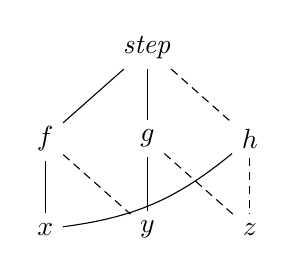
\begin{tikzpicture}[baseline=(cy.base)]
  \node (cx) at (0,0) {$x$};
  \node (cy) at (1.3,0) {$y$};
  \node (cz) at (2.6,0) {$z$};
  \node (cf) at (0,1.15) {$f$};
  \node (cg) at (1.3,1.15) {$g$};
  \node (ch) at (2.6,1.15) {$h$};
  \node (cs) at (1.3,2.3) {$\mathit{step}$};
  \draw (cf) -- (cx);
  \draw[densely dashed] (cf) -- (cy);
  \draw (cg) -- (cy);
  \draw[densely dashed] (cg) -- (cz);
  \draw (ch) to[bend left=16] (cx);
  \draw[densely dashed] (ch) -- (cz);
  \draw (cs) -- (cf);
  \draw (cs) -- (cg);
  \draw[densely dashed] (cs) -- (ch);
\end{tikzpicture}
\caption{The 2-cell \texttt{step} of the \texttt{Compose} type, twice
over. Left, the pasting diagram: \texttt{step} rewrites the pasted
path \texttt{f \#0 g} into \texttt{h}. Right, the shape it realizes,
an oriented graded poset drawn as a Hasse diagram: solid covering
edges are input faces ($\partial^-$, the \texttt{BdryIn} rows of
\S\ref{sec:gt-alifib-tier2}), dashed ones output faces ($\partial^+$,
\texttt{BdryOut}). Seven cells in grades of sizes $(3,3,1)$, nine
signed edges --- row for row, the complex the transcripts below carry.}
\label{fig:gt-alifib-step}
\end{figure}

Save the listing as \texttt{compose.ali} at the repository root. The
export bridge (built once with \texttt{cargo build --release} in
\path{vendor/alifib}; \S\ref{sec:gt-alifib-convert} gives it a proper
tour) elaborates the file with the engine's own loader and interpreter
--- boundaries checked, shapes realized --- and \texttt{--check} stops
there, printing a summary. The first line is the file's module root, a
type holding nothing here; the one map on the second line is the
identity self-map the engine mints for every type, which
\S\ref{sec:gt-alifib-convert} returns to:

\begin{Verbatim}[fontsize=\small,frame=leftline,rulecolor=\color{accentmid},framesep=3mm,xleftmargin=3mm]
$ vendor/alifib/target/release/alifib-export compose.ali --check
compose.ali: type  — 0 generators, 0 diagrams, 0 maps (0 holes), 0 complexes
compose.ali: type Compose — 7 generators, 0 diagrams, 1 maps (0 holes),
                            7 complexes
warnings: 0
\end{Verbatim}

\noindent Ill-formed input stops at this gate with the engine's own
diagnostics: declare \texttt{oops:\ f f -> f} (pasting \texttt{f}
onto itself along a boundary the types do not share) and the export
exits nonzero with ``\texttt{Failed to paste diagrams: boundaries do
not match}'', pointing at the offending span. Nothing unchecked
reaches the rows.

Dropping \texttt{--check} emits the interchange document
(\S\ref{sec:gt-alifib-convert} specifies it):

\begin{Verbatim}[fontsize=\small,frame=leftline,rulecolor=\color{accentmid},framesep=3mm,xleftmargin=3mm]
$ vendor/alifib/target/release/alifib-export compose.ali -o compose.json
wrote compose.json (7616 bytes)
\end{Verbatim}

\noindent Two slices of it, whitespace refolded to the book's measure
and content bytes as emitted --- the \texttt{step} generator, whose
source is the paste tree itself:

\begin{Verbatim}[fontsize=\small,frame=leftline,rulecolor=\color{accentmid},framesep=3mm,xleftmargin=3mm]
{ "name": "step",
  "dim": 2,
  "src": { "paste": 0, "l": { "gen": "f" }, "r": { "gen": "g" } },
  "tgt": { "gen": "h" } }
\end{Verbatim}

\noindent and the materialized shape of \texttt{step}, the right-hand
panel of Figure~\ref{fig:gt-alifib-step} as data (grades bottom-up;
\texttt{faces\_in[d-1][p]} lists the input faces, at grade $d{-}1$, of
the $p$-th cell at grade $d$, as indices into the canonical order):

\begin{Verbatim}[fontsize=\small,frame=leftline,rulecolor=\color{accentmid},framesep=3mm,xleftmargin=3mm]
{ "of": { "kind": "generator", "name": "step" },
  "sizes": [3, 3, 1],
  "faces_in":  [ [[0], [1], [0]],  [[0, 1]] ],
  "faces_out": [ [[1], [2], [2]],  [[2]]    ],
  "labels": [ ["x", "y", "z"], ["f", "g", "h"], ["step"] ] }
\end{Verbatim}

The import half turns the document into instance rows against the
Alifib theory. Watch the paste tree become constructor rows, with
hash-consing visible (\texttt{f} and \texttt{g} each occur once as
leaves, then the paste refers back to them):

\begin{Verbatim}[fontsize=\small,frame=leftline,rulecolor=\color{accentmid},framesep=3mm,xleftmargin=3mm]
$ python3 theories/tools/alifib_interop.py import compose.json \
    -o compose.rows.txt
wrote compose.rows.txt (221 lines)
\end{Verbatim}

\noindent Operations 44 through 50 of that listing:

\begin{Verbatim}[fontsize=\small,frame=leftline,rulecolor=\color{accentmid},framesep=3mm,xleftmargin=3mm]
op[ 44] elta sort=G<alifib/Diag>                        // Diag: f
op[ 45] funa fun=G<alifib/dGen> args=[L16] value=L44    // dGen f
op[ 46] elta sort=G<alifib/Diag>                        // Diag: g
op[ 47] funa fun=G<alifib/dGen> args=[L20] value=L46    // dGen g
op[ 48] elta sort=G<alifib/Diag>                        // Diag: (f #0 g)
op[ 49] funa fun=G<alifib/dPaste> args=[nat:0, L44, L46] value=L48
op[ 50] funa fun=G<alifib/Gen/src> args=[L28] value=L48 // src of step
\end{Verbatim}

\noindent and, at the listing's tail, the last three of the figure's
nine signed edges --- the top cell's own --- as boundary rows
(\texttt{L196} names the \texttt{step} cell; \texttt{L181},
\texttt{L186}, \texttt{L191} the \texttt{f}, \texttt{g}, \texttt{h}
cells):

\begin{Verbatim}[fontsize=\small,frame=leftline,rulecolor=\color{accentmid},framesep=3mm,xleftmargin=3mm]
op[207] rela rel=G<alifib/BdryIn> args=[L196, L181]
op[208] rela rel=G<alifib/BdryIn> args=[L196, L186]
op[209] rela rel=G<alifib/BdryOut> args=[L196, L191]
\end{Verbatim}

\noindent These are ordinary instance rows; engine instruments consume
them as such. The census verb, for one, seeds them under the theory
and analyses which function symbols' merges the derivation leans on
(a dry-run instrument, it desugars the function symbols the chase
bridge refuses --- its first line counts them):

\begin{Verbatim}[fontsize=\small,frame=leftline,rulecolor=\color{accentmid},framesep=3mm,xleftmargin=3mm]
$ geolog census theories/Alifib.geolog --rows compose.rows.txt
merge-reliance census — 1 file(s), 1 rows listing(s), 24 arrow(s) desugared
  ⋮
seeds: 44 elements, 166 rows
\end{Verbatim}

Finally, back out. The projection inverts the import, and the
\texttt{.ali} renderer turns the interchange back into source, with
every paste parenthesized so the engine re-reads the same binary
trees:

\begin{Verbatim}[fontsize=\small,frame=leftline,rulecolor=\color{accentmid},framesep=3mm,xleftmargin=3mm]
$ python3 theories/tools/alifib_interop.py project compose.rows.txt \
    -o back.json
$ python3 theories/tools/alifib_interop.py to-ali back.json -o back.ali
$ sed -n 5,14p back.ali
@Type
Compose <<= {
    x,
    y,
    z,
    f: x -> y,
    g: y -> z,
    h: x -> z,
    step: (f #0 g) -> h
}
$ python3 theories/tools/alifib_interop.py accept compose.ali
ACCEPT: CLEAN
\end{Verbatim}

\noindent The \texttt{accept} verb at the end is the round trip run as
a test, both directions at once; the next subsection says what it
checks.

\subsection{Converting data to and from alifib}
\label{sec:gt-alifib-convert}

This subsection is written for readers who keep data in alifib's own
formats --- its maintainers first among them --- and want the crossing
stated precisely: where the bridge lives, what travels over it, the
commands for each direction, what survives a round trip, and what is
checked on the way in. The reward for crossing is everything this
chapter has shown: types, diagrams, proofs, and their realized shapes
as rows in a substrate with signed content-addressed commits, merge by
set union, derived provenance views like \texttt{Diag/uses}, and a
schema that is data in the same log.

\paragraph{The bridge, and why it lives where it does.}
alifib's structural core (paste trees, oriented graded posets) is a
private module, and the engine's own output surfaces render for
display: boundary expressions as strings, paste chains flattened, no
incidence tables. A faithful exporter therefore has to live
\emph{inside} the engine crate, where crate-private data is reachable,
and drive the interpreter itself; anything else would be a
reimplementation, trusted precisely where it should not be. The
geolog-alpha repository vendors a pinned copy of the engine carrying
that exporter as one additive module
(\path{vendor/alifib}; provenance, upstream commit, and the complete
patch list are in \path{vendor/alifib/VENDOR.md}, and the patch is
written to be upstreamable as-is). The bridge builds from a fresh
clone:

\begin{Verbatim}[fontsize=\small,frame=leftline,rulecolor=\color{accentmid},framesep=3mm,xleftmargin=3mm]
$ cd vendor/alifib && cargo build --release
$ ./target/release/alifib-export --help
usage: alifib-export <file.ali> [--type NAME] [--all-modules]
                     [--complexes none|gens|named|all] [-o OUT] [--check]
\end{Verbatim}

\noindent By default the root file's module is exported with every
named type, and shapes are materialized for every generator and named
diagram; \texttt{--complexes none} keeps the export purely syntactic,
\texttt{--type} restricts to one type, \texttt{--all-modules} includes
what the file \texttt{include}s. Output is deterministic --- two runs
are byte-identical --- because every collection rides a canonical
order: generators ascending by (dimension, name), which is also a
dependency-safe declaration order, since a generator's boundary leaves
are strictly lower-dimensional; diagrams and maps by name; cells in
the engine's own normalization order.

\paragraph{The interchange document.} One JSON document per export,
versioned by its first key. In sketch (field names exact, values
elided):

\begin{Verbatim}[fontsize=\small,frame=leftline,rulecolor=\color{accentmid},framesep=3mm,xleftmargin=3mm]
{ "alifib_interop": 1,
  "generator": "alifib-export (geolog interop bridge)",
  "source": "<root file basename>",
  "modules": [
    { "path": "<path relative to the root file>",
      "types": [
        { "name": "...",
          "generators": [ { "name", "dim", "src"?, "tgt"? } ],
          "diagrams":   [ { "name", "dim", "tree" } ],
          "maps":       [ { "name", "domain", "images", "holes" } ],
          "complexes":  [ { "of", "sizes",
                            "faces_in", "faces_out", "labels" } ] } ] } ],
  "warnings": [ "..." ] }
\end{Verbatim}

\noindent A generator's \texttt{src}/\texttt{tgt} are present iff its
dimension is positive. \texttt{diagrams} carries the type's named
diagrams: \texttt{let} bindings and proofs stored from interactive
sessions. A map's \texttt{domain} is either
\texttt{\{"type":\ t\}} or \texttt{\{"module":\ m\}}; its
\texttt{images} are filled assignments, its \texttt{holes} the open
ones, each hole optionally carrying a conditional image and
metavariable boundary trees. A complex records whose shape it is
(\texttt{of}), its per-grade extents (\texttt{sizes}), both signed
face lists indexed as in \S\ref{sec:gt-alifib-e2e}, and per-cell
generator labels. Boundary terms and diagram trees share one grammar,
four node shapes in total:

\begin{Verbatim}[fontsize=\small,frame=leftline,rulecolor=\color{accentmid},framesep=3mm,xleftmargin=3mm]
{"gen": "f"}                      a single-cell diagram
{"paste": k, "l": t1, "r": t2}    t1 #k t2 -- the engine's own binary
                                  node, never flattened or re-associated
{"hole": "g"}                     a map hole's metavariable (appears
                                  only in hole boundary terms)
{"labels": [...], "ldim": n}      loud fallback for a diagram with no
                                  paste history at its top dimension;
                                  counted in warnings, not a term
\end{Verbatim}

\paragraph{Into geolog.} \texttt{import} compiles a dump to instance
rows; \texttt{--type} restricts, as with the exporter:

\begin{Verbatim}[fontsize=\small,frame=leftline,rulecolor=\color{accentmid},framesep=3mm,xleftmargin=3mm]
$ python3 theories/tools/alifib_interop.py import mine.json -o mine.rows.txt
\end{Verbatim}

\noindent The output is a plain-text listing of numbered operations in
the meta-schema's instance vocabulary, three kinds in all:
\texttt{elta} mints an element of a sort, \texttt{funa} asserts a
function row, \texttt{rela} a relation row. Arguments are literals
(\texttt{nat:0}, \texttt{str:"step"}) or backreferences
(\texttt{L48} names the element minted by operation 48; forward
references are ill-formed by construction). The
\texttt{G<alifib/\ldots>} tokens cite the Alifib theory's declaration
identities, so the listing is meaningful against any store holding
that revision. Each distinct paste tree becomes one \texttt{Diag}
element per type, however often it recurs --- the hash-consing of
\S\ref{sec:gt-alifib-tier1}, performed at import time. The importer
runs a structural self-check before writing (every reference points
backward and at an element; every external token lies within the
Alifib signature) and stamps the verdict in the header; the committed
listings under
\path{theories/generated/} are regeneration-checked against their
generators by the repository's check script, so drift between tool and
artifact is loud.

What admission means, in layers: the importer's self-check is the
shallow layer; the theory's demand axioms are the deep one. Every
imported element owes the judgments of
\S\ref{sec:gt-alifib-tier1} --- well-formedness, pastability,
roundness --- and those side-conditions are discharged by the engine,
which is to say: by re-elaboration. Running
\texttt{alifib-export mine.ali --check} \emph{is} the decision
procedure, executed on the way out of alifib, before the rows exist;
the incidence laws (sign-disjointness and parity) are additionally
checkable without the engine, and
\texttt{alifib\_interop.py verify-scx mine.json} does so directly on a
dump. Engine instruments consume the rows today
(\texttt{geolog check} for theory-side conformance,
\texttt{geolog census} for merge-reliance analysis, the
meta-rows loader in the repository's test suite for loader
conformance), and the one-verb facade of \S\ref{sec:gt-log} seals
theory \emph{sources}; an admission seam that seals imported instance
rows like these behind the same store is the piece still in design
tense, and this paragraph sheds the qualifier when it lands.

\paragraph{Out of geolog.} Two verbs invert the import:

\begin{Verbatim}[fontsize=\small,frame=leftline,rulecolor=\color{accentmid},framesep=3mm,xleftmargin=3mm]
$ python3 theories/tools/alifib_interop.py project mine.rows.txt -o back.json
$ python3 theories/tools/alifib_interop.py to-ali back.json -o back.ali
\end{Verbatim}

\noindent \texttt{project} rebuilds an interchange document from rows.
It is deterministic, total on the import's image, and loud off it:
unknown functions or sorts, dangling references, a \texttt{Diag} with
no constructor row, a map marked total with absent images (inside the
database that state is a judged, standing debt; the exporter never
emits it, so the projection holds it off the image), an index at or
beyond its grade's extent, a count mismatch between declared extents
and cells, non-adjacent boundary rows --- each is a named rejection,
not a silent drop. \texttt{to-ali} renders an interchange document as
\texttt{.ali} source: every paste fully parenthesized, so the engine
re-reads the same binary trees; identifiers outside alifib's lexical
grammar sanitized deterministically, with the name map recorded in the
header comment; maps emitted as module-level \texttt{let total}
declarations; and the identity self-map the engine generates for every
type is skipped, since elaboration regenerates it. The acceptance
judge for this direction is alifib itself: the round-trip witness
re-elaborates the rendered source with the engine's own parser and
loader and compares the re-export against the original document.

\paragraph{What survives, what degrades.} Surviving a full round trip,
per type, structurally intact: generator names, dimensions, and
boundary trees as exact binary pastes (no re-association); named
diagrams and their assemblies; map images and holes, as assignments
over the domain's generators; complexes cell for cell --- extents,
both signed face lists, labels. Degrading, each by design and each
documented in the tools' headers: map \emph{names} are not carried by
rows, so maps re-emerge under fresh names; a conditional image (one
recorded on a hole but awaiting boundary resolution) degrades to a
plain hole, and the engine re-derives the constraint on
re-elaboration; maps
whose domain is a whole module are skipped with a note, the module
system being surface elaboration that the interpreter flattens before
the proof theory begins; display metadata (\texttt{index} blocks) does
not travel; execution traces sit outside interchange version~1 ---
the \texttt{Trace} sort of \S\ref{sec:gt-alifib-tier1} is the landing
site reserved for them.

\paragraph{The acceptance harness.} Both witnesses run as one verb per
file (\texttt{accept}, as in \S\ref{sec:gt-alifib-e2e}), and over a
fixed ten-file corpus spanning the shipped examples' feature surface
--- abstract machines, higher-categorical developments, hole
workflows, simplicial complexes; the parity measurement of
\S\ref{sec:gt-alifib-tier2} separately covered all twenty-two files:

\begin{Verbatim}[fontsize=\small,frame=leftline,rulecolor=\color{accentmid},framesep=3mm,xleftmargin=3mm]
$ python3 theories/tools/alifib_interop.py accept-corpus
BinaryNat.ali: CLEAN
EckmannHilton.ali: CLEAN
  ⋮
Hole_examples.ali: CLEAN
LambdaSigma.ali: CLEAN
CORPUS: 10/10 clean
\end{Verbatim}

\noindent Witness one: export, import, project; the projection must
reproduce the interchange up to the documented degradations. Witness
two: export, render to \texttt{.ali}, re-elaborate with the engine,
re-export; the second document must match the first up to the recorded
name map --- boundary trees, hole sets, and complexes cell for cell.
Every round-trip claim this subsection has made is one of those
comparisons or one of the named rejections. Readers extending the
interchange --- traces are the obvious next passenger --- extend the
witnesses first; the harness is the contract.

\section{The scorecard}
\label{sec:gt-scorecard}

Where the SQL stack wins today, plainly: \textbf{Throughput and
maturity.} Kafka moves gigabytes per second and Feldera maintains
complex view cascades incrementally, while this preview's chase is a
correct, differentially-tested reference implementation whose
incrementality so far covers violation views only. \textbf{Aggregates
and windows.} Streaming SQL's core vocabulary, not native to the
geometric fragment (explicit constructions or the ground seam, at
tutorial scale). \textbf{Operations.} The surrounding decade of
connectors, monitoring, and hiring.

Where geolog wins, plainly: \textbf{Views you can audit.} Derived
state is entailment, re-derivable and checkable from the log by a
third party, with provenance; there is no fold code to believe.
\textbf{Merge without a protocol.} Set union plus re-derivation,
order-free, defined for every pair of replicas, with no per-type merge
design and no rebalance to choreograph. \textbf{Judgments over
exceptions.} Invalid states and pending choices are typed, reportable
data with the violated axiom attached, rather than code paths.
\textbf{Writers you can hold to account.} Signatures,
content-addressing, and structural equivocation detection are the data
model, not an add-on. \textbf{One substrate.} Schema, extension,
annotation, and migration are rows in the same log they govern; there
is no registry to drift.

Compose the two lists and the position comes out plain. At this
preview, geolog has the right shape for systems of record where
auditability, principled merge, and schema-as-data carry the value, at
volumes where a reference-grade engine suffices. It is also built
deliberately so that the fast paths can arrive without the trust story
changing (the lane law; the kernels repository).

\section{Composing systems, and where QTSL begins}
\label{sec:gt-onward}

The order flow of this chapter is one system. The book's larger
programme composes systems, with shared boundaries, wiring diagrams,
and the population and fusion of components, and it states
\emph{temporal} claims about the composites. Those claims are not of
the form ``no cancelled order has shipped''; that is a state property,
and you watched a denial say it. They look instead like ``every placed
order is shipped or refunded within thirty days, with probability at
least $p$.'' Those are claims the chase alone cannot check and the
event log alone cannot even state. Stating them is QTSL's job, and
certifying them against models is the rest of this book: the systems
vocabulary in chapter~\ref{ch:qtsl-mathematical-models}, the
composition patterns in chapter~\ref{ch:qtsl-composition-patterns},
and the zero-to-certificate path in chapter~\ref{ch:qtsl-quickstart}.
You now hold the substrate they all stand on: a log whose truth is
structural, tables that are theorems, and a schema that is data.

